\documentclass[../Lab.tex]{subfiles}
\begin{document}

%----------------------------------------------------------------------------------------
%	PROCEDURES
%----------------------------------------------------------------------------------------
\section{Procedures}
\subsection{Set Up One}

 \begin{figure}[H] % [H] forces the figure to be placed exactly where it appears in the text
	\centering % Horizontally center the figure
	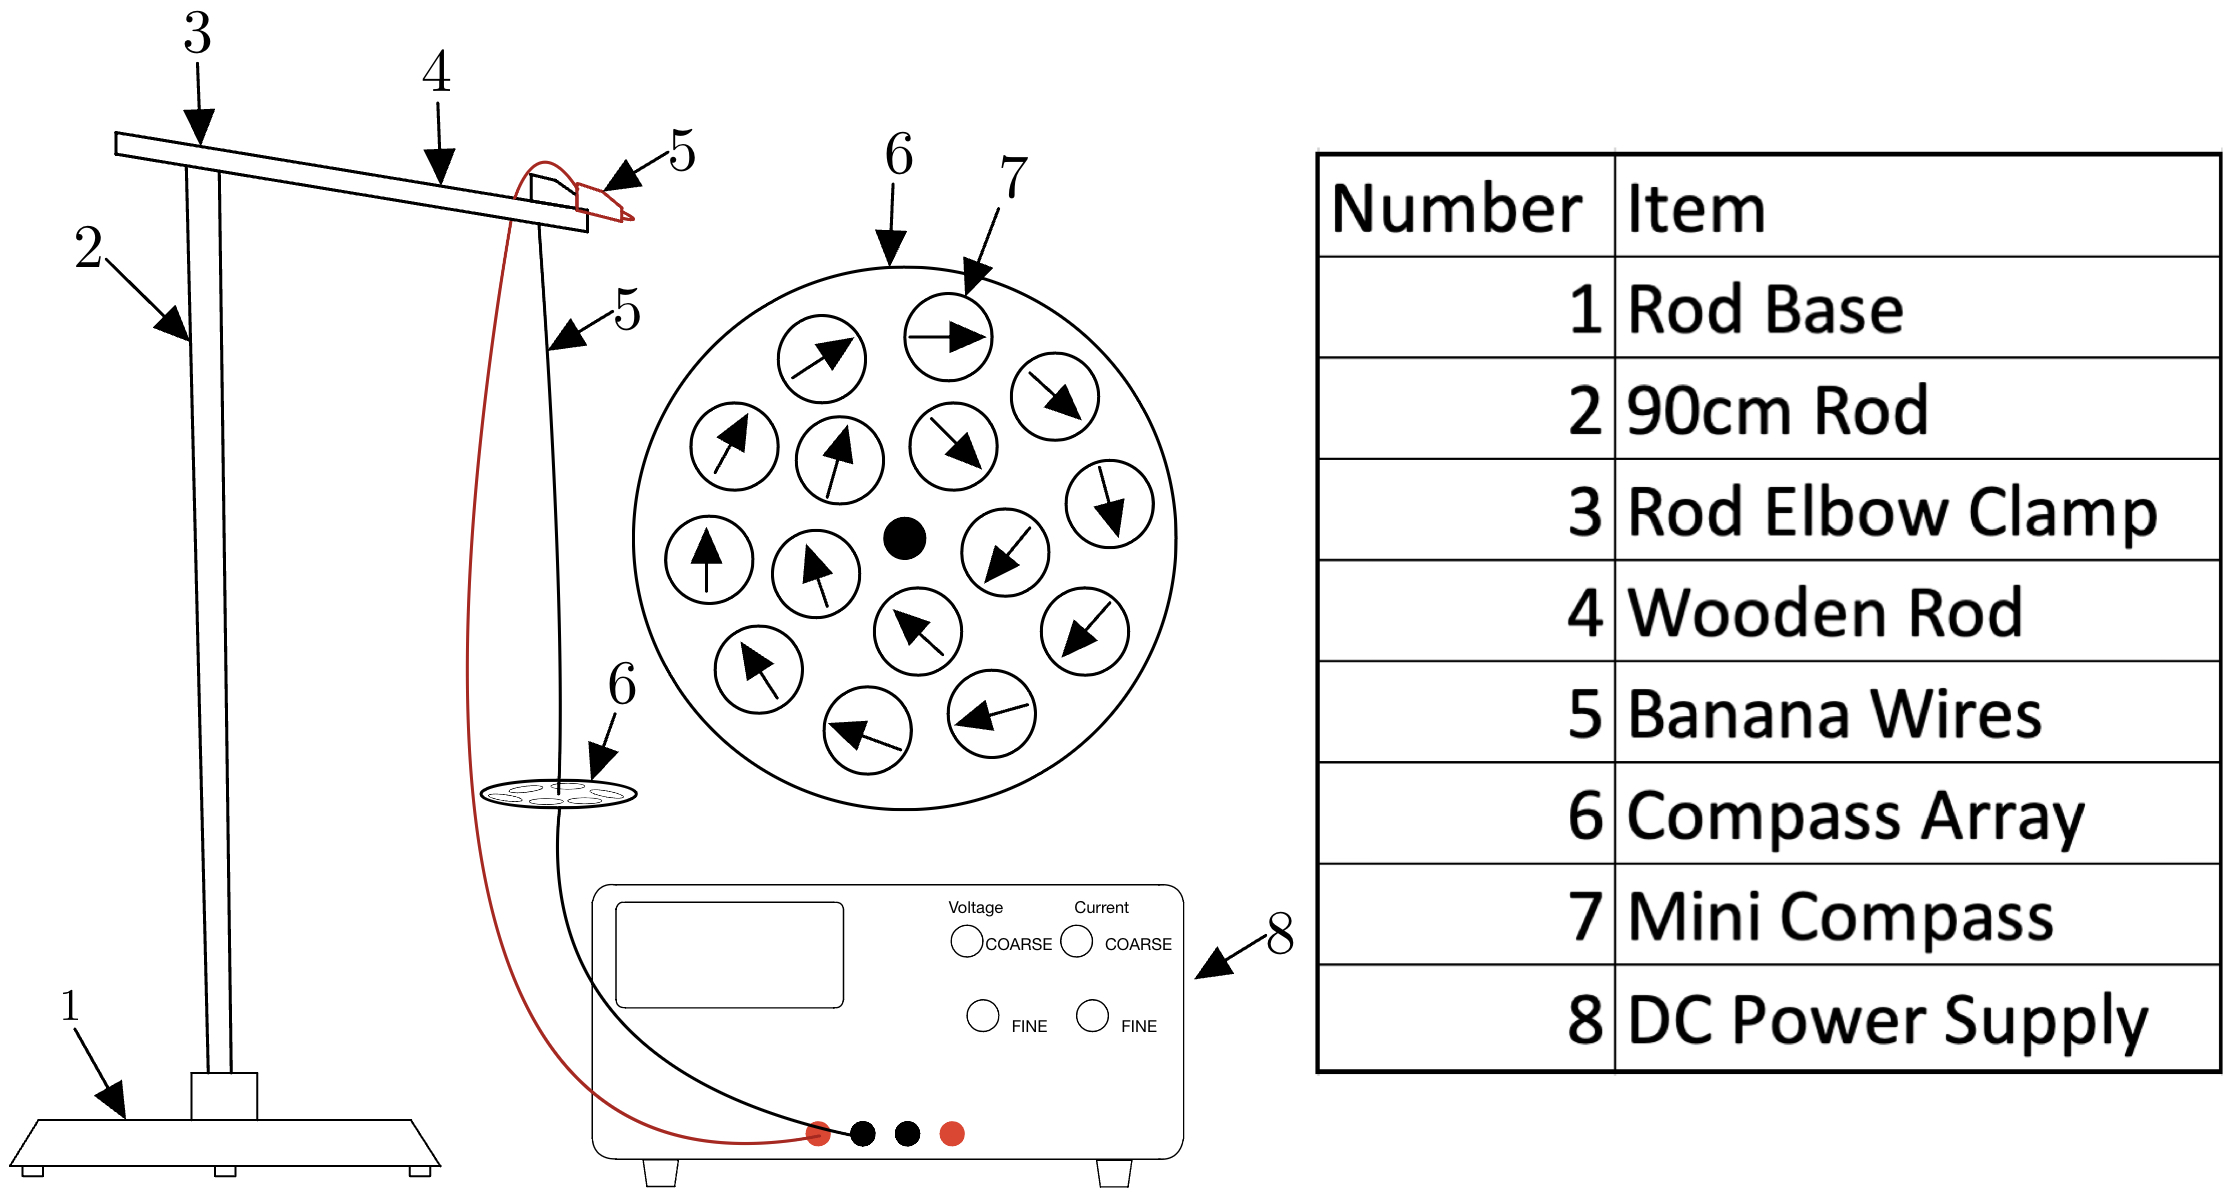
\includegraphics[width=1\textwidth]{ Lab 9 Procedures Diagram Part A.png} % Include the figure
	\caption{Dependence of B on I Experimental Setup}
\end{figure}

\begin{enumerate}[1)]
    \item Example instructions step: Connect the BNC cable that corresponds to channel 1 of the Oscilloscope to the BNC cable of the function generator by using banana cables. Remember to match the color coding by connecting the Red banana cable to the Red connection point, and the Black banana cable to the Black connection point. Prioritize safety when making all connections.
    \item Continue instructions.
    \item Continue instructions.
    
\end{enumerate}


\subsection{Setup Two}
\begin{enumerate}[1)]
    \item Continue instructions.
    \item Continue instructions.
    \item Continue instructions.
    
\end{enumerate}

\end{document}

\HectorHatesTrees